\documentclass{beamer}
\mode<presentation>


\usepackage[brazil]{babel}
\usepackage[utf8]{inputenc}

\usepackage{amsfonts}
\usepackage{amssymb}
\usepackage{amsmath}
\usepackage{ae}
\usepackage{graphicx,color}
\usepackage[all]{xy}
\usepackage{empheq}
\usepackage{fancybox}
\usepackage{textcomp}
\usepackage[all]{xy}
\usepackage{textpos}
\usepackage{multicol}
\usepackage{cancel}
\usepackage{listings}
\usepackage{xcolor}
\usepackage{tikz}
\usepackage{enumerate}

\usetikzlibrary{matrix}
\usetikzlibrary{arrows}
\usetikzlibrary{shapes,snakes}
\usetikzlibrary{calc}


\newcommand{\floor}[1]{$\lfloor$ #1 $\rfloor$}

\newcommand\Fontvi{\fontsize{9}{7.2}\selectfont}



\usetheme{Boadilla}

\newcommand{\PC}[1]{\ensuremath{\left(#1\right)}}


\newcommand*{\colorboxed}{}
\def\colorboxed#1#{%
  \colorboxedAux{#1}%
}
\newcommand*{\colorboxedAux}[3]{%
  % #1: optional argument for color model
  % #2: color specification
  % #3: formula
  \begingroup
    \colorlet{cb@saved}{.}%
    \color#1{#2}%
    \boxed{%
      \color{cb@saved}%
      #3%
    }%
  \endgroup
}



\title {Olimpíada Brasileira de Informática 2018 \\Modalidade Iniciação \\ Nível Júnior \\ Fase Local}

\author[Projeto Semeando Talentos]{ Projeto Semeando Talentos$^{1}$  }

\institute[UFC]{$^{1}$Universidade Federal do Ceará - Campus de Quixadá\\}
\date{}
\AtBeginSection[]
{
  \begin{frame}<beamer>{}
    \small
    \tableofcontents[currentsection,currentsubsection]
  \end{frame}
}
\begin{document}

\begin{frame}
	\titlepage
\end{frame}

%%%%%%%%%%%%%%%%%%%%%%%%%%%%%%%%%%%%%%%%%%%%%%%%%%%%%%%%%%%%%%%%%%%%

\begin{frame}{Troco}
\textit{No Brasil há notas de R\$ 100, R\$ 50, R\$ 20, R\$ 10, R\$5 e R\$2.}



\textbf{Questão 1.} Qual o menor número de notas que um comerciante pode dar como troco, usando apenas notas, para um cliente que deu três notas de R\$ 100 para pagar uma mercadoria que custa R\$ 201?
\begin{enumerate}
 \item[(A)] 5
 \item[(B)] 6
 \item[(C)] 7
 \item[(D)] 8
 \item[(E)] 9
\end{enumerate}

\end{frame}

%%%%%%%%%%%%%%%%%%%%%%%%%%%%%%%%%%%%%%%%%%%%%%%%%%%%%%%%%%%%%%%%%%%%
\begin{frame}{Solução (Troco)}
\begin{itemize}
Para tentarmos formar o troco (R\$ 99,00) com o menor número de notas possíveis, vamos utilizar primeiramente os maiores valores e depois os menores. 
\end{itemize}

\pause

\begin{figure}[tb]
\begin{center}
	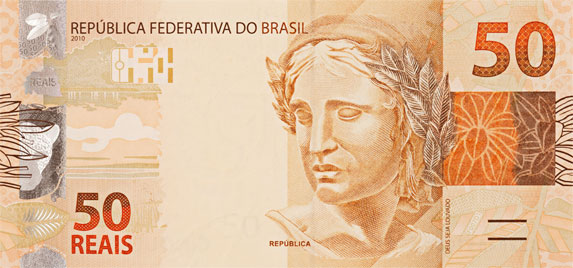
\includegraphics[height=2cm]{50.jpg} \pause \quad
	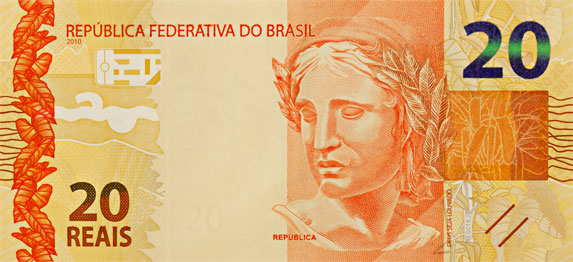
\includegraphics[height=2cm]{20.jpg}
\end{center}
\end{figure}

\pause

\begin{figure}[tb]
\begin{center}
	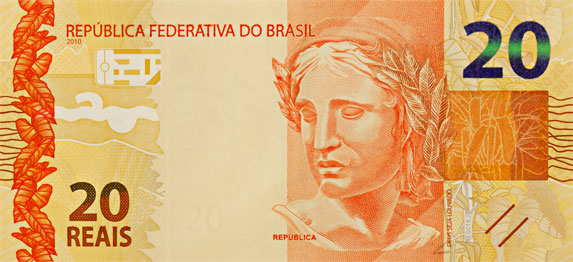
\includegraphics[height=2cm]{20.jpg} \pause \quad
	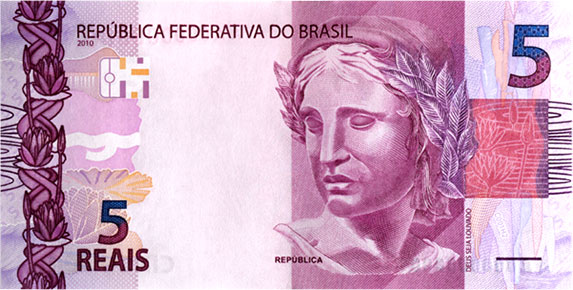
\includegraphics[height=2cm]{5.jpg}
\end{center}
\end{figure}

\pause

\begin{figure}[tb]
\begin{center}
	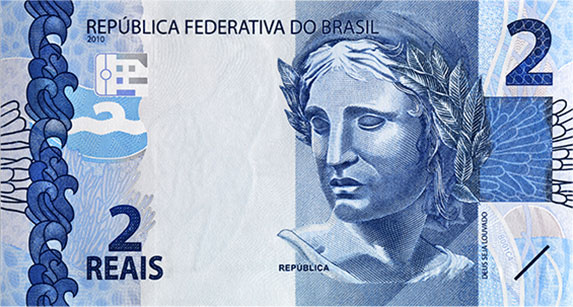
\includegraphics[height=2cm]{2.jpg} \pause \quad
	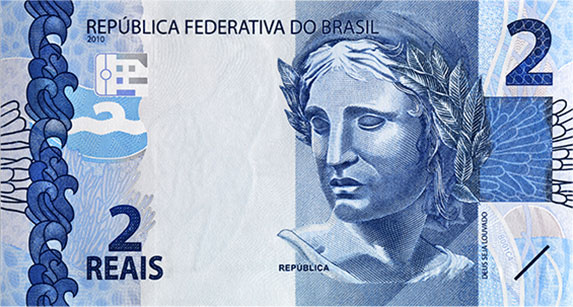
\includegraphics[height=2cm]{2.jpg}
\end{center}
\end{figure}





\end{frame}

%%%%%%%%%%%%%%%%%%%%%%%%%%%%%%%%%%%%%%%%%%%%%%%%%%%%%%%%%%%%%%%%%%%%
\begin{frame}{Troco}
\textit{No Brasil há notas de R\$ 100, R\$ 50, R\$ 20, R\$ 10, R\$5 e R\$2.}



\textbf{Questão 1.} Qual o menor número de notas que um comerciante pode dar como troco, usando apenas notas, para um cliente que deu três notas de R\$ 100 para pagar uma mercadoria que custa R\$ 201?
\begin{enumerate}
 \item[(A)] 5
 \item[(B)]\textbf{6}
 \item[(C)] 7
 \item[(D)] 8
 \item[(E)] 9
\end{enumerate}

\end{frame}

\begin{frame}{Quadrados}
\textit{No Brasil há notas de R\$ 100, R\$ 50, R\$ 20, R\$ 10, R\$5 e R\$2.}



\textbf{Questão 2.} Qual o menor número de notas que um cliente pode usar para pagar uma mercadoria que custa R\$ 201, usando apenas notas?
\begin{enumerate}
 \item[(A)] 5
 \item[(B)] 6
 \item[(C)] 7
 \item[(D)] 8
 \item[(E)] 9
\end{enumerate}

\end{frame}

%%%%%%%%%%%%%%%%%%%%%%%%%%%%%%%%%%%%%%%%%%%%%%%%%%%%%%%%%%%%%%%%%%%%

\begin{frame}{Solução (Quadrados)}
\textit{No Brasil há notas de R\$ 100, R\$ 50, R\$ 20, R\$ 10, R\$5 e R\$2.}
\begin{itemize}
    \item Vamos continuar utilizando notas de maiores valores para formar o valor. Se optarmos pelas de menor valor, o número de notas irá ser maior.
    \item Se utilizarmos duas notas de R\$ 100,00 não teremos como completar o valor, veja:
\end{itemize}

\begin{figure}[tb]
\begin{center}
	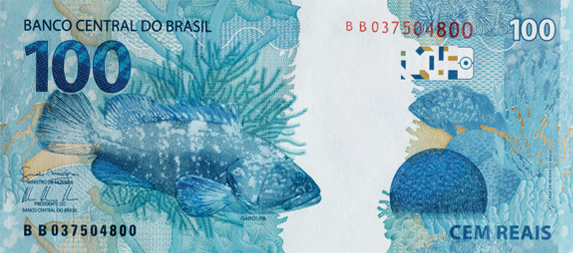
\includegraphics[height=2cm]{100.jpg} \pause \quad
	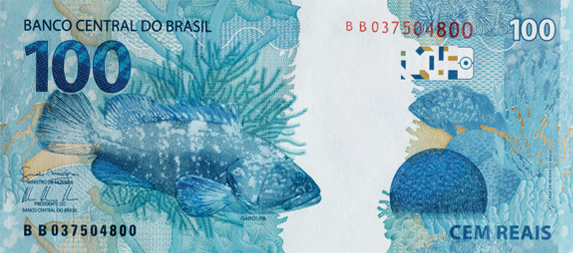
\includegraphics[height=2cm]{100.jpg}
\end{center}
\end{figure}

\begin{figure}[tb]
\begin{center}
	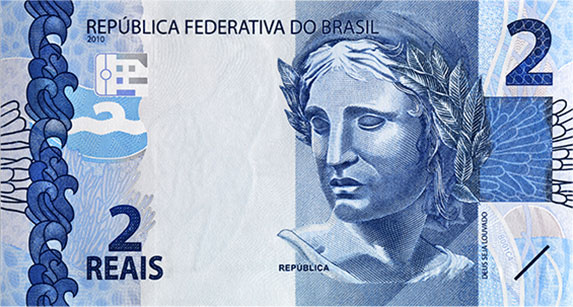
\includegraphics[height=2cm]{2.jpg} 
\end{center}
\end{figure}

\end{frame}

%%%%%%%%%%%%%%%%%%%%%%%%%%%%%%%%%%%%%%%%%%%%%%%%%%%%%%%%%%%%%%%%%%%%
\begin{frame}{Solução (Quadrados)}
\textit{No Brasil há notas de R\$ 100, R\$ 50, R\$ 20, R\$ 10, R\$5 e R\$2.}
\begin{itemize}
    \item Portanto, vamos tentar utilizar um nota de R\$100,00 e formar o valor restante com notas de menor valor.
\end{itemize}

\begin{figure}[tb]
\begin{center}
	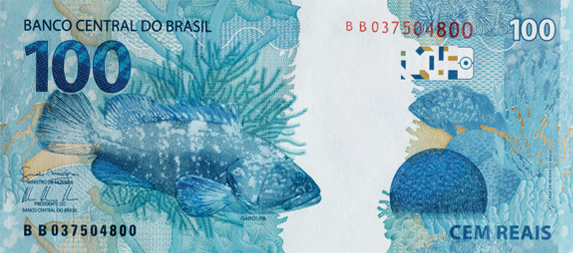
\includegraphics[height=1cm]{100.jpg} \pause \quad
	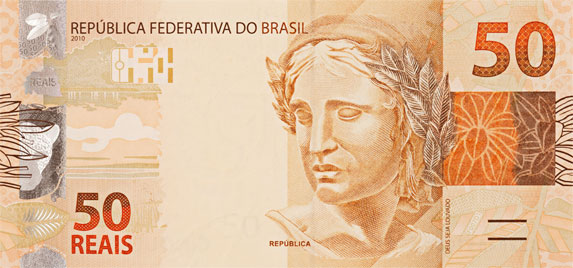
\includegraphics[height=1cm]{50.jpg}
\end{center}
\end{figure}
\pause 
\begin{figure}[tb]
\begin{center}
	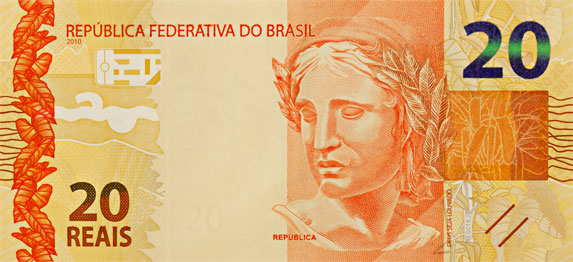
\includegraphics[height=1cm]{20.jpg}  \pause \quad
	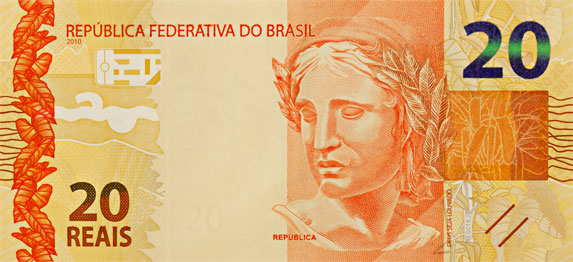
\includegraphics[height=1cm]{20.jpg}
\end{center}
\end{figure}
\pause 
\begin{figure}[tb]
\begin{center}
	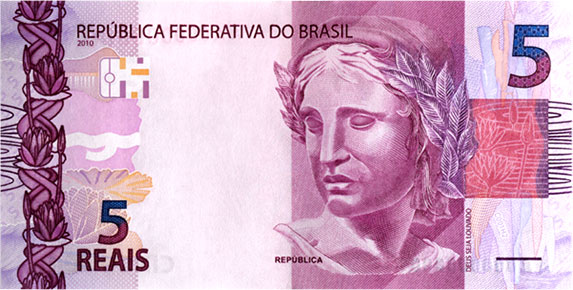
\includegraphics[height=1cm]{5.jpg}  \pause \quad 
	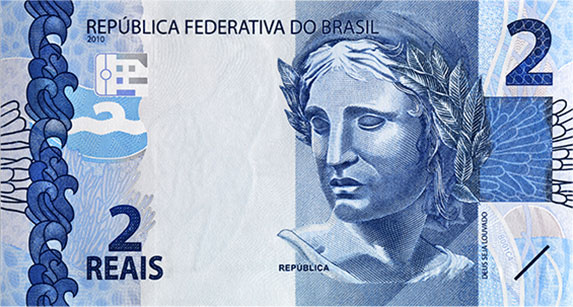
\includegraphics[height=1cm]{2.jpg} \quad
\end{center}
\end{figure}
 \pause 
\begin{figure}[tb]
\begin{center}
	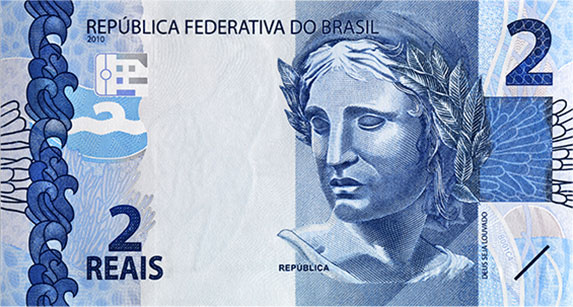
\includegraphics[height=1cm]{2.jpg} \quad
	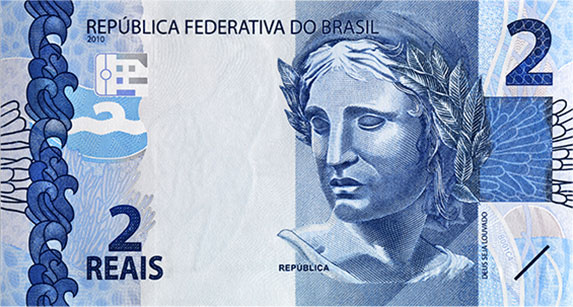
\includegraphics[height=1cm]{2.jpg}
\end{center}
\end{figure}

\end{frame}


%%%%%%%%%%%%%%%%%%%%%%%%%%%%%%%%%%%%%%%%%%%%%%%%%%%%%%%%%%%%%%%%%%%%
\begin{frame}{Quadrados}
\textit{No Brasil há notas de R\$ 100, R\$ 50, R\$ 20, R\$ 10, R\$5 e R\$2.}



\textbf{Questão 2.} Qual o menor número de notas que um cliente pode usar para pagar uma mercadoria que custa R\$ 201, usando apenas notas?
\begin{enumerate}
 \item[(A)] 5
 \item[(B)] 6
 \item[(C)] 7
 \item[(D)] \textbf{8}
 \item[(E)] 9
\end{enumerate}

\end{frame}

%%%%%%%%%%%%%%%%%%%%%%%%%%%%%%%%%%%%%%%%%%%%%%%%%%%%%%%%%%%%%%%%%%%%

\begin{frame}{Quadrados}
Uma linha de quadrados é construída usando palitos de fósforo, como mostrado na figura abaixo.


\begin{figure}[ht]
\centering
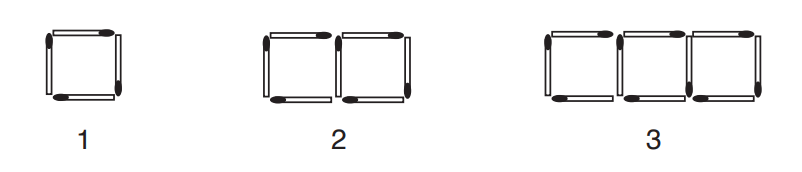
\includegraphics[width=.9\textwidth]{fosforos.png}
\label{fig:exampleFig2}
\end{figure}

\textbf{Questão 3.} Quantos palitos são necessários para construir a linha que tem cinco quadrados?

\begin{enumerate}
 \item[(A)] 10
 \item[(B)] 12
 \item[(C)] 13
 \item[(D)] 16
 \item[(E)] 20
\end{enumerate}
\end{frame}


%%%%%%%%%%%%%%%%%%%%%%%%%%%%%%%%%%%%%%%%%%%%%%%%%%%%%%%%%%%%%%%%%%%%

\begin{frame}{Quadrados}
A partir da linha de 3 quadrados, vamos adicionar um fósforo de cada vez até que se formem todos os 5
\begin{figure}[ht]
\centering
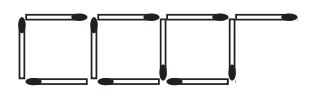
\includegraphics[width=.6\textwidth]{f1.png}
\label{fig:exampleFig2}
\end{figure}
\end{frame}

%%%%%%%%%%%%%%%%%%%%%%%%%%%%%%%%%%%%%%%%%%%%%%%%%%%%%%%%%%%%%%%%%%%%

\begin{frame}{Solução (Quadrados)}
Para isso, vamos adicionar um fósforo de cada vez até que se formem os 
5 quadrados. 
\begin{figure}[ht]
\centering
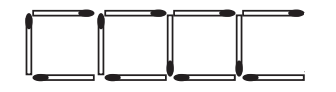
\includegraphics[width=.6\textwidth]{f2.png}
\label{fig:exampleFig2}
\end{figure}
\end{frame}

%%%%%%%%%%%%%%%%%%%%%%%%%%%%%%%%%%%%%%%%%%%%%%%%%%%%%%%%%%%%%%%%%%%%


\begin{frame}{Solução (Quadrados)}
Para isso, vamos adicionar um fósforo de cada vez até que se formem os 
5 quadrados. 
\begin{figure}[ht]
\centering
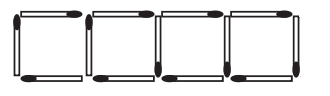
\includegraphics[width=.6\textwidth]{f3.png}
\label{fig:exampleFig2}
\end{figure}
\end{frame}

%%%%%%%%%%%%%%%%%%%%%%%%%%%%%%%%%%%%%%%%%%%%%%%%%%%%%%%%%%%%%%%%%%%%


\begin{frame}{Solução (Quadrados)}
Colocando os fósforos da mesma forma que vimos antes, chegaremos na linha de 5 quadrados como queríamos:  
\begin{figure}[ht]
\centering
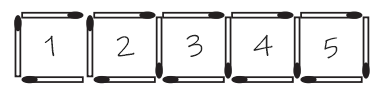
\includegraphics[width=.6\textwidth]{f4.png}
\label{fig:exampleFig2}
\end{figure}
\end{frame}

%%%%%%%%%%%%%%%%%%%%%%%%%%%%%%%%%%%%%%%%%%%%%%%%%%%%%%%%%%%%%%%%%%%%


\begin{frame}{Solução (Quadrados)}
 
\begin{figure}[ht]
\centering
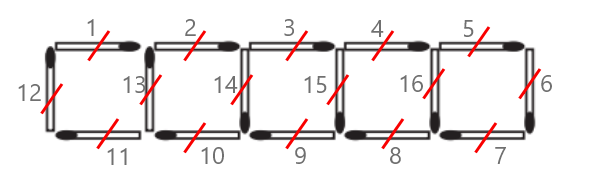
\includegraphics[width=.7\textwidth]{solucao.png}
\label{fig:exampleFig2}
\end{figure}
Resposta: 16 palitos de fósforo \\
\end{frame}

%%%%%%%%%%%%%%%%%%%%%%%%%%%%%%%%%%%%%%%%%%%%%%%%%%%%%%%%%%%%%%%%%%%%

\begin{frame}{Solução (Quadrados)}
\begin{itemize}
\item O ideal é achar um padrão para calcular a quantidade para qualquer número de quadrados.
\item Podemos observar que para formar 1 quadrado precisamos de 4 palitos. Para formar 2 quadrados, precisamos de 7 palitos. 
\end{itemize}
\end{frame}

\begin{frame}{Solução (Quadrados)}


\begin{figure}[ht]
\centering
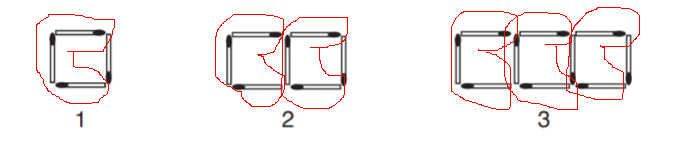
\includegraphics[width=.6\textwidth]{q2.png}
\label{fig:exampleFig2}
\end{figure}

Portanto, podemos calcular a quantidade de palitos a partir do número de quadrados utilizando a seguinte fórmula: 

\begin{equation*}
    p = (q \ast 3) + 1
\end{equation*}

Sendo \textbf{p} a quantidade de \textit{palitos} e \textbf{q} a quantidade de \textit{quadrados}.
\end{frame}

%%%%%%%%%%%%%%%%%%%%%%%%%%%%%%%%%%%%%%%%%%%%%%%%%%%%%%%%%%%%%%%%%%%%


\begin{frame}{Solução (Quadrados)}
\begin{equation*}
    p = (q \ast 3) + 1
\end{equation*}

\begin{figure}[ht]
\centering
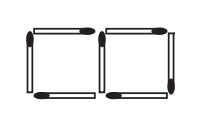
\includegraphics[width=.2\textwidth]{2qua.png}
\label{fig:exampleFig2}
\end{figure}

\begin{equation*}
    p = (2 \ast 3) + 1 = 6 + 1 =7
\end{equation*}

\begin{figure}[ht]
\centering
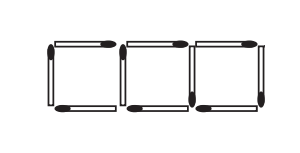
\includegraphics[width=.3\textwidth]{3qua.png}
\label{fig:exampleFig2}
\end{figure}

\begin{equation*}
    p = (3 \ast 3) + 1 = 9 + 1 = 10
\end{equation*}

\end{frame}

%%%%%%%%%%%%%%%%%%%%%%%%%%%%%%%%%%%%%%%%%%%%%%%%%%%%%%%%%%%%%%%%%%%%



\begin{frame}{Solução (Quadrados)}
\begin{figure}[ht]
\centering
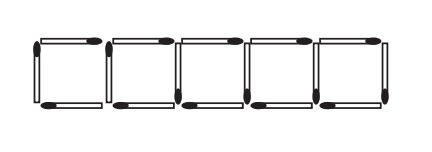
\includegraphics[width=.6\textwidth]{5qua.png}
\label{fig:exampleFig2}
\end{figure}

\begin{equation*}
    p = (q \ast 3) + 1 
\end{equation*}

\begin{equation*}
    p = (5 \ast 3) + 1 = 15 + 1 = 16
\end{equation*}

\end{frame}

%%%%%%%%%%%%%%%%%%%%%%%%%%%%%%%%%%%%%%%%%%%%%%%%%%%%%%%%%%%%%%%%%%%%

\begin{frame}{Questão 2 (2018) - Iniciação Nível Júnior}

Uma linha de quadrados é construída usando palitos de fósforo, como mostrado na figura abaixo.

\begin{figure}[ht]
\centering
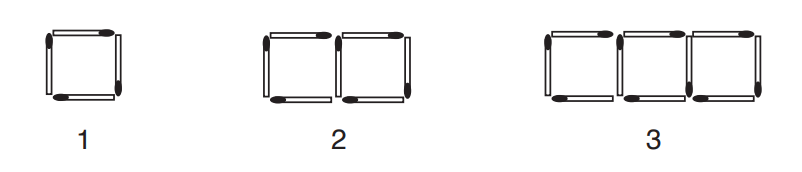
\includegraphics[width=.9\textwidth]{fosforos.png}
\label{fig:exampleFig2}
\end{figure}

\textbf{Questão 3.} Quantos palitos são necessários para construir a linha que tem cinco quadrados?

\begin{enumerate}
 \item[(A)] 10
 \item[(B)] 12
 \item[(C)] 13
 \item[(D)] \textbf{16}
 \item[(E)] 20
\end{enumerate}
\end{frame}
%%%%%%%%%%%%%%%%%%%%%%%%%%%%%%%%%%%%%%%%%%%%%%%%%%%%%%%%%%%%%%%%%%%%
\begin{frame}{Quadrados}

\textbf{Questão 4.} Quantos palitos são necessários
para construir a linha com 21 quadrados?
\begin{enumerate}[(A)]
    \item 64
    \item 67
    \item 75
    \item 84
    \item 91
\end{enumerate}

\end{frame}

%%%%%%%%%%%%%%%%%%%%%%%%%%%%%%%%%%%%%%%%%%%%%%%%%%%%%%%%%%%%%%%%%%%%

\begin{frame}{Quadrados}

Agora podemos utilizar a fórmula que encontramos. Dessa vez, vamos substituir o valor de 21 quadrado para encontrar a quantidade necessária de palitos, portanto temos:

\begin{equation*}
    p = (q \ast 3) + 1
\end{equation*}
Para q = 21,
\begin{equation*}
    p = (21 \ast 3) + 1
\end{equation*}

\begin{equation*}
    p = (63) + 1
\end{equation*}
Logo, 
\begin{equation*}
    p = 64
\end{equation*}
\end{frame}

%%%%%%%%%%%%%%%%%%%%%%%%%%%%%%%%%%%%%%%%%%%%%%%%%%%%%%%%%%%%%%%%%%%%

\begin{frame}{Quadrados}

\textbf{Questão 4.} Quantos palitos são necessários
para construir a linha com 21 quadrados?
\begin{enumerate}[(A)]
    \item \textbf{64}
    \item 67
    \item 75
    \item 84
    \item 91
\end{enumerate}

\end{frame}

%%%%%%%%%%%%%%%%%%%%%%%%%%%%%%%%%%%%%%%%%%%%%%%%%%%%%%%%%%%%%%%%%%%%

\begin{frame}{Quadrados}

\textbf{Questão 5.} Quantos quadrados tem a linha com o maior número de quadrados que é possível construir com uma caixa de palitos de  fósforo que contém 42 palitos?

\begin{enumerate}[(A)]
    \item 10
    \item 11
    \item 12
    \item 13
    \item 14
\end{enumerate}
\end{frame}

%%%%%%%%%%%%%%%%%%%%%%%%%%%%%%%%%%%%%%%%%%%%%%%%%%%%%%%%%%%%%%%%%%%%
\begin{frame}{Solução (Quadrados)}

Utilizando nossa fórmula, vamos descobrir quantos quadrados podem ser formados com 42 palitos:
\begin{equation*}
    p = (q \ast 3) + 1
\end{equation*}
\pause
    \begin{equation*}
        42 = (q \ast 3) + 1
    \end{equation*}
\pause
    \begin{equation*}
       (q \ast 3) = 41
    \end{equation*}
\pause
    \begin{equation*}
      q = 41 \div 3
    \end{equation*}
\pause
    \begin{equation*}
    q = 13,66
    \end{equation*}
\pause
    Como não existem 13,66 quadrados, podemos assumir que para 42 palitos, é possível formar uma linha de \textbf{13 quadrados}. 
\end{frame}

%%%%%%%%%%%%%%%%%%%%%%%%%%%%%%%%%%%%%%%%%%%%%%%%%%%%%%%%%%%%%%%%%%%%

\begin{frame}{Solução - (Quadrados)}

\textbf{Questão 5.} Quantos quadrados tem a linha com o maior número de quadrados que é possível construir com uma caixa de palitos de  fósforo que contém 42 palitos?

\begin{enumerate}[(A)]
    \item 10
    \item 11
    \item 12
    \item \textbf{13}
    \item 14
\end{enumerate}
\end{frame}
 
 
%%%%%%%%%%%%%%%%%%%%%%%%%%%%%%%%%%%%%%%%%%%%%%%%%%%%%%%%%%%%%%%%%%%%

\begin{frame}{Cerca de Madeira}

Maria está construindo uma cerca com postes e traves de madeira, como nos diagramas abaixo. Cada trave tem um metro de comprimento. Vamos desconsiderar a largura dos postes, e dessa forma a cerca do diagrama 1 tem um metro de comprimento, a cerca do diagrama 2 tem dois metros de comprimento e a cerca do diagrama 3 tem três metros de comprimento.

\begin{figure}[ht]
\centering
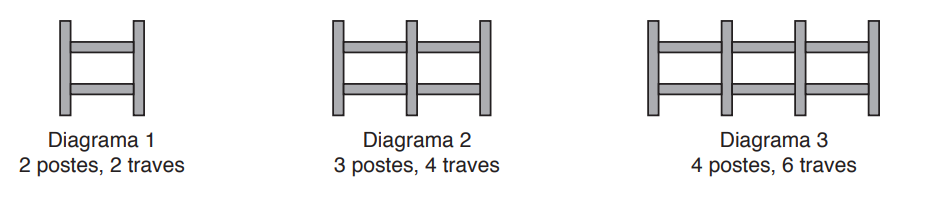
\includegraphics[width=.9\textwidth]{diagramas.png}
\label{fig:exampleFig2}
\end{figure}

\end{frame}
%%%%%%%%%%%%%%%%%%%%%%%%%%%%%%%%%%%%%%%%%%%%%%%%%%%%%%%%%%%%%%%%%%%%

\begin{frame}{Cerca de Madeira}
\textbf{Questão 6}. Quantas traves terá uma cerca com
seis postes?

\begin{enumerate}[(A)]
    \item 6
    \item 10
    \item 12
    \item 14
    \item 16
\end{enumerate}

\end{frame}
%%%%%%%%%%%%%%%%%%%%%%%%%%%%%%%%%%%%%%%%%%%%%%%%%%%%%%%%%%%%%%%%%%%%
\begin{frame}{Solução (Cerca de Madeira)}

Para 6 postes, temos a seguinte representação:
\begin{figure}[ht]
\centering
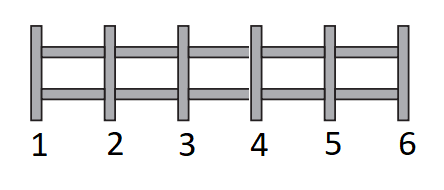
\includegraphics[width=.6\textwidth]{postes.png}
\label{fig:exampleFig2}
\end{figure}

\begin{itemize}
    \item Podemos notar cada poste é comporta 2 traves.\\
     \item Já a última trave não comporta, ela apenas é usada para completar a última certa. \\
     \item Portanto, podemos assumir a seguinte função genérica para qualquer quantidade de cerca:
     \begin{equation*}
        traves(n) =  (n \ast 2)  - 2
     \end{equation*}
     Sendo \textit{n} a quantidade de postes.
\end{itemize}


\end{frame}

%%%%%%%%%%%%%%%%%%%%%%%%%%%%%%%%%%%%%%%%%%%%%%%%%%%%%%%%%%%%%%%%%%%%
\begin{frame}{Solução (Cerca de Madeira)}
\begin{figure}[ht]
\centering
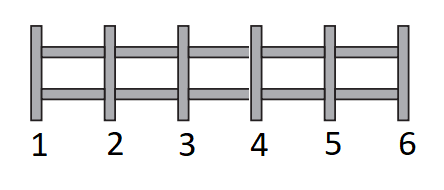
\includegraphics[width=.6\textwidth]{postes.png}
\label{fig:exampleFig2}
\end{figure}
Portanto, para n = 6, temos:
    \begin{equation*}
        traves(6) = 6 \ast 2 - 2
    \end{equation*}
Logo,
    \begin{equation*}
        traves(6) = 10 
    \end{equation*}

\end{frame}
%%%%%%%%%%%%%%%%%%%%%%%%%%%%%%%%%%%%%%%%%%%%%%%%%%%%%%%%%%%%%%%%%%%%
\begin{frame}{Cerca de Madeira}
\textbf{Questão 6}. Quantas traves terá uma cerca com
seis postes?

\begin{enumerate}[(A)]
    \item 6
    \item \textbf{10}
    \item 12
    \item 14
    \item 16
\end{enumerate}

\end{frame}

%%%%%%%%%%%%%%%%%%%%%%%%%%%%%%%%%%%%%%%%%%%%%%%%%%%%%%%%%%%%%%%%%%%%
\begin{frame}{Cerca de Madeira}
\textbf{Questão 7}. Se Maria tem exatamente 27 traves
e 17 postes, quantos metros de comprimento tem
a maior cerca ela pode construir?

\begin{enumerate}[(A)]
    \item 13
    \item 16
    \item 17
    \item 26
    \item 27
\end{enumerate}

\end{frame}
%%%%%%%%%%%%%%%%%%%%%%%%%%%%%%%%%%%%%%%%%%%%%%%%%%%%%%%%%%%%%%%%%%%%
\begin{frame}{Solução (Cerca de Madeira)}

Como o número de traves sempre deve ser par, vamos considerar que Maria poderá utilizar no máximo 26 traves. Com isso, vamos calcular o número de postes que serão utilizados para construir a cerca:
    \begin{equation*}
        traves(n) = n \ast 2 - 2
    \end{equation*}
    \begin{equation*}
       n \ast 2 = 2 + 26 
    \end{equation*}
     \begin{equation*}
       n = 28\div2
    \end{equation*}
     \begin{equation*}
       n = 14
    \end{equation*}
    Dos 17 postes disponíveis, Maria só poderá utilizar 14. 


\end{frame}



%%%%%%%%%%%%%%%%%%%%%%%%%%%%%%%%%%%%%%%%%%%%%%%%%%%%%%%%%%%%%%%%%%%%
\begin{frame}{Cerca de Madeira}

Lembrando que cada trave possui 1m, podemos descobrir o comprimento da cerca a partir do número de postes. Temos que em metros, o comprimento será
\begin{equation*}
    comprimento(n) = n - 1
\end{equation*}
onde $n$ é o número de postes.


Agora que temos o número de postes utilizadas, podemos calcular o comprimento da cerca:


    \begin{equation*}
       comprimento(14) = 14 - 1
    \end{equation*}
    \begin{equation*}
       comprimento(14) = 13  
    \end{equation*}
     
\end{frame}

%%%%%%%%%%%%%%%%%%%%%%%%%%%%%%%%%%%%%%%%%%%%%%%%%%%%%%%%%%%%%%%%%%%%
\begin{frame}{Cerca de Madeira}
\textbf{Questão 7}. Se Maria tem exatamente 27 traves
e 17 postes, quantos metros de comprimento tem
a maior cerca ela pode construir?

\begin{enumerate}[(A)]
    \item \textbf{13}
    \item 16
    \item 17
    \item 26
    \item 27
\end{enumerate}

\end{frame}

%%%%%%%%%%%%%%%%%%%%%%%%%%%%%%%%%%%%%%%%%%%%%%%%%%%%%%%%%%%%%%%%%%%%
\begin{frame}{Cerca de Madeira}
\textbf{Questão 8}. Cada poste custa R\$ 10,00 e cada trave custa R\$ 5,00. Qual o custo de uma cerca com onze metros de comprimento?


\begin{enumerate}[(A)]
    \item R\$ 180,00
    \item R\$ 190,00
    \item R\$ 200,00
    \item R\$ 210,00
    \item R\$ 230,00
\end{enumerate}

\end{frame}
%%%%%%%%%%%%%%%%%%%%%%%%%%%%%%%%%%%%%%%%%%%%%%%%%%%%%%%%%%%%%%%%%%%%
\begin{frame}{Cerca de Madeira}
\begin{itemize}
    \item Se uma cerca possui onze metros de comprimento, então a quantidade de postes é 12.
    \pause 
    \item A quantidade de traves para $n$ postes é $2*n-2$, ou seja, precisaremos  $2 \ast 12 - 2  = 22$ traves.

    \item Se cada poste custa R\$10,00, então o valor gasto será:
\begin{equation*}
   R\$10\ast 12 = R\$120,00
\end{equation*}
\pause
    \item Se cada trave custa R\$5,00, então o valor gasto será:
\begin{equation*}
    R\$5\ast 22 = R\$110,00
\end{equation*}
\end{itemize}
\pause
Logo, o custo total de uma cerca com onze metros de comprimento será:
\begin{equation*}
    R\$120,00 + R\$110,00 = R\$230,00
\end{equation*}

\end{frame}

%%%%%%%%%%%%%%%%%%%%%%%%%%%%%%%%%%%%%%%%%%%%%%%%%%%%%%%%%%%%%%%%%%%%
\begin{frame}{Cerca de Madeira}
\textbf{Questão 8}. Cada poste custa R\$ 10,00 e cada trave custa R\$ 5,00. Qual o custo de uma cerca com onze metros de comprimento?


\begin{enumerate}[(A)]
    \item R\$ 180,00
    \item R\$ 190,00
    \item R\$ 200,00
    \item R\$ 210,00
    \item \textbf{R\$ 230,00}
\end{enumerate}

\end{frame}

%%%%%%%%%%%%%%%%%%%%%%%%%%%%%%%%%%%%%%%%%%%%%%%%%%%%%%%%%%%%%%%%%%%%
\begin{frame}{Viagens de Ônibus}
Uma cidade tem exatamente cinco bairros: Areias, Brejo, Centro, Delta e Embu. Existem exatamente seis linhas de ônibus ligando os bairros, com os seguintes preços de passagens (o preço é o
mesmo para a ida ou a volta):
\begin{center}
\begin{enumerate}[(1)]
\item Centro – Brejo: R\$ 9,00 
\item Delta – Embu: R\$ 3,00
\item Centro – Embu: R\$ 3,00
\item Areias – Brejo: R\$ 4,00
\item Centro – Delta: R\$ 1,00 
\item Areias – Delta: R\$ 2,00
\end{enumerate}
\end{center}

\end{frame}
%%%%%%%%%%%%%%%%%%%%%%%%%%%%%%%%%%%%%%%%%%%%%%%%%%%%%%%%%%%%%%%%%%%%
\begin{frame}{Viagens de Ônibus}
\textbf{Questão 9}. Qual o menor valor total em passagens para ir de ônibus de Embu para Brejo?


\begin{enumerate}[(A)]
    \item R\$ 5,00
    \item R\$ 7,00
    \item R\$ 9,00
    \item R\$ 13,00
    \item R\$ 14,00
\end{enumerate}

\end{frame}

%%%%%%%%%%%%%%%%%%%%%%%%%%%%%%%%%%%%%%%%%%%%%%%%%%%%%%%%%%%%%%%%%%%%
\begin{frame}{Viagens de Ônibus - Solução}
\begin{figure}[ht]
\centering
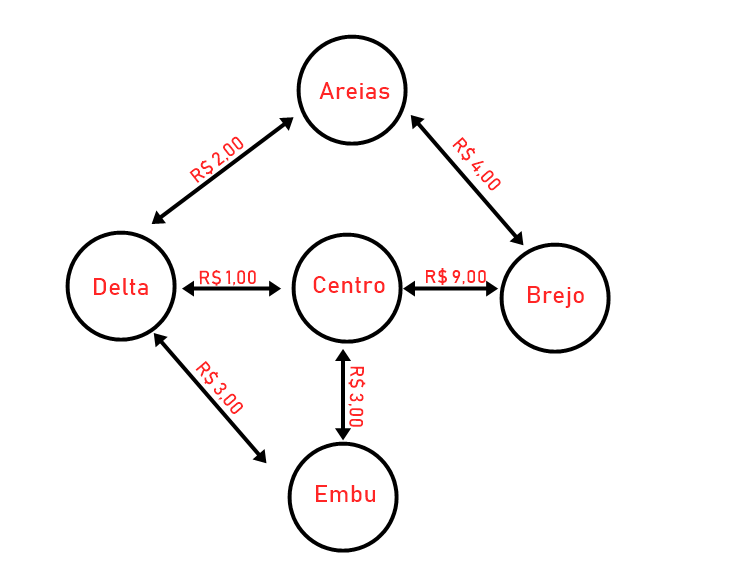
\includegraphics[width=.8\textwidth]{onibus.png}
\label{fig:exampleFig2}
\end{figure}
\end{frame}

%%%%%%%%%%%%%%%%%%%%%%%%%%%%%%%%%%%%%%%%%%%%%%%%%%%%%%%%%%%%%%%%%%%%
\begin{frame}{Viagens de Ônibus - Solução}
\begin{figure}[ht]
\centering
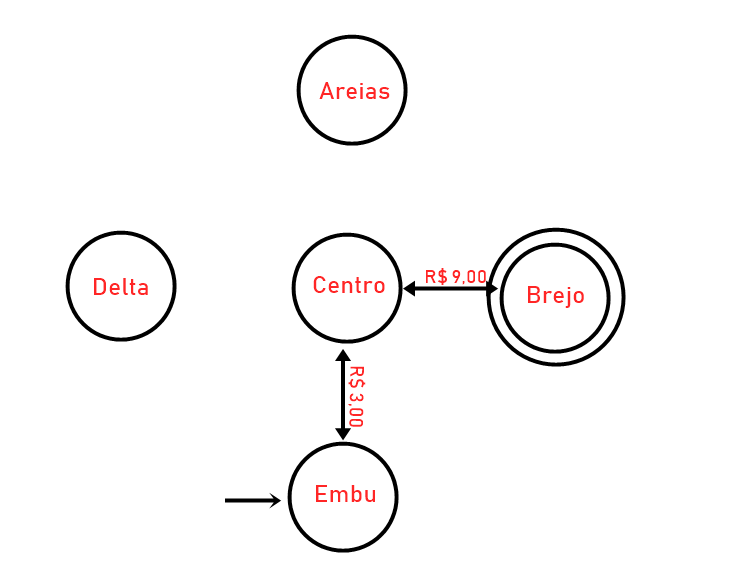
\includegraphics[width=.7\textwidth]{caminho1.png}
\label{fig:exampleFig2}
\end{figure}
\begin{equation*}
    Total = R\$3,00 + R\$9,00 = R\$12,00  
\end{equation*}

\end{frame}


%%%%%%%%%%%%%%%%%%%%%%%%%%%%%%%%%%%%%%%%%%%%%%%%%%%%%%%%%%%%%%%%%%%%
\begin{frame}{Viagens de Ônibus - Solução}
\begin{figure}[ht]
\centering
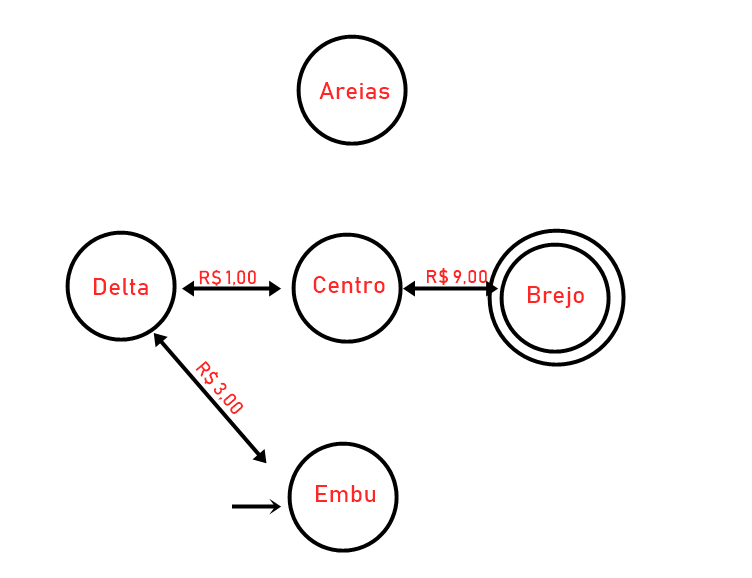
\includegraphics[width=.7\textwidth]{caminho2.png}
\label{fig:exampleFig2}
\end{figure}

\begin{equation*}
    Total = R\$3,00 + R\$1,00 + R\$9,00 = R\$13,00  
\end{equation*}

\end{frame}


%%%%%%%%%%%%%%%%%%%%%%%%%%%%%%%%%%%%%%%%%%%%%%%%%%%%%%%%%%%%%%%%%%%%
\begin{frame}{Viagens de Ônibus - Solução}
\begin{figure}[ht]
\centering
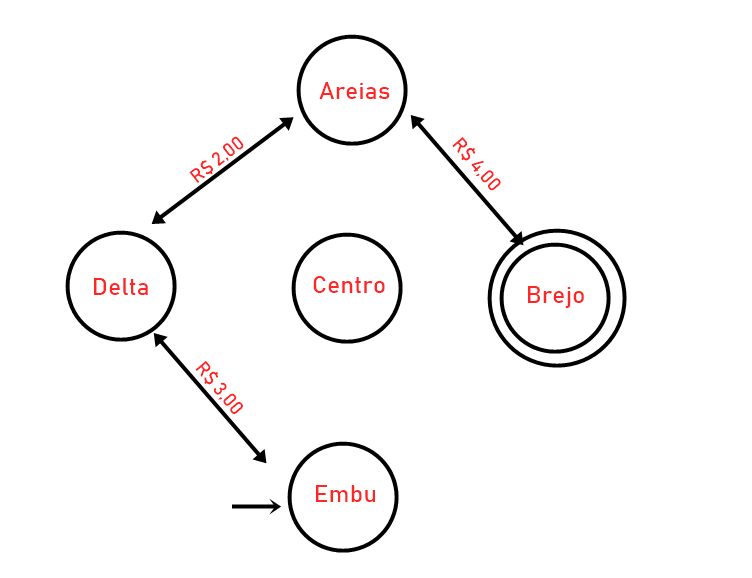
\includegraphics[width=.7\textwidth]{caminho3.png}
\label{fig:exampleFig2}
\end{figure}
\begin{equation*}
    Total = R\$3,00 + R\$2,00 + R\$4,00 = R\$9,00  
\end{equation*}
\end{frame}

%%%%%%%%%%%%%%%%%%%%%%%%%%%%%%%%%%%%%%%%%%%%%%%%%%%%%%%%%%%%%%%%%%%%
\begin{frame}{Viagens de Ônibus}
\textbf{Questão 10}. Aos domingos o preço da passagem
Centro – Brejo é promocional e custa metade do
preço normal. Nesse caso, qual o menor valor em
passagens para ir de ônibus de Brejo para Delta?

\begin{enumerate}[(A)]
    \item R\$ 2,00
    \item R\$ 4,50
    \item R\$ 5,50
    \item R\$ 6,00
    \item R\$ 9,50
\end{enumerate}
\end{frame}


%%%%%%%%%%%%%%%%%%%%%%%%%%%%%%%%%%%%%%%%%%%%%%%%%%%%%%%%%%%%%%%%%%%%
\begin{frame}{Solução (Viagens de Ônibus)}
Com o valor promocional alterado, temos as as seguintes rotas:

\begin{figure}[ht]
\centering
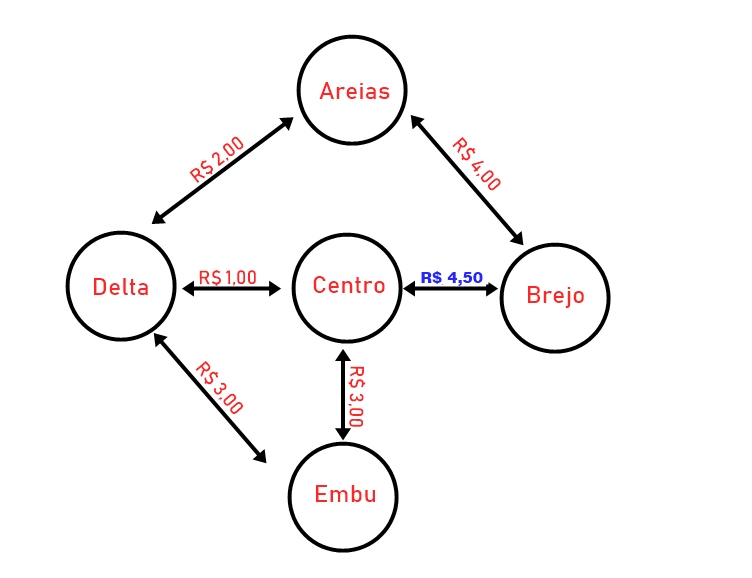
\includegraphics[width=.7\textwidth]{onibuspromocional.png}
\label{fig:exampleFig2}
\end{figure}

Em seguida, vamos visualizar os possível caminhos para Brejo – Delta. 

\end{frame}

\begin{frame}{Solução (Viagens de Ônibus)}
\begin{figure}[ht]
\centering
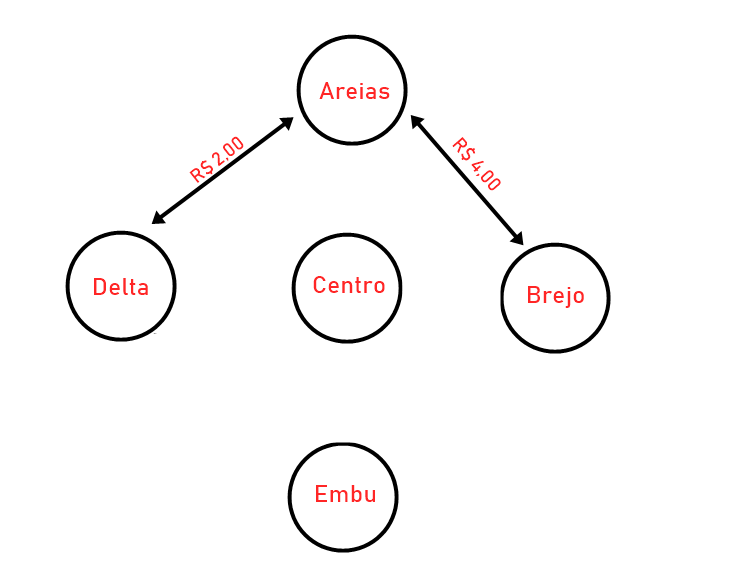
\includegraphics[width=.8\textwidth]{DB1.png}
\label{fig:exampleFig2}
\end{figure}
\begin{equation*}
    \textbf{Total} = R\$2,00 + R\$4,00 = \textbf{R\$6,00}
\end{equation*}

\end{frame}

\begin{frame}{Solução (Viagens de Ônibus)}

\begin{figure}[ht]
\centering
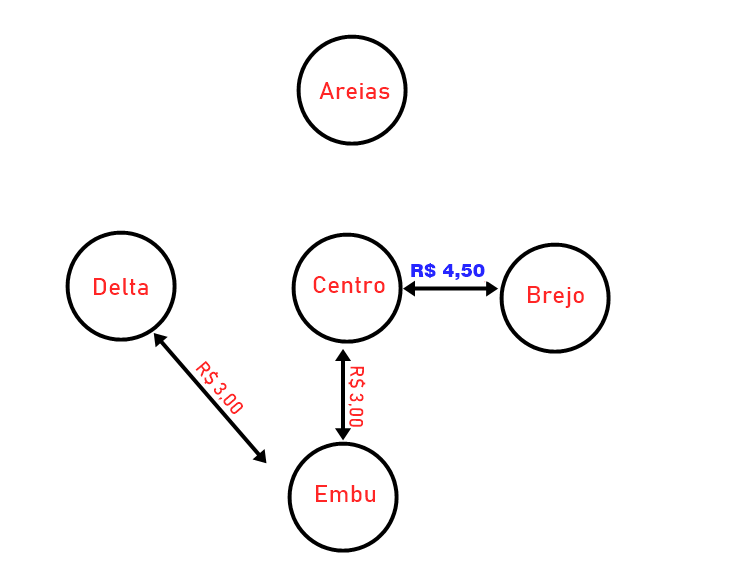
\includegraphics[width=.8\textwidth]{DB2.png}
\label{fig:exampleFig2}
\end{figure}
\begin{equation*}
    \textbf{Total} = R\$3,00 + R\$3,00 + R\$4,50 = \textbf{R\$10,50}
\end{equation*}

\end{frame}

\begin{frame}{Solução (Viagens de Ônibus)}
\begin{figure}[ht]
\centering
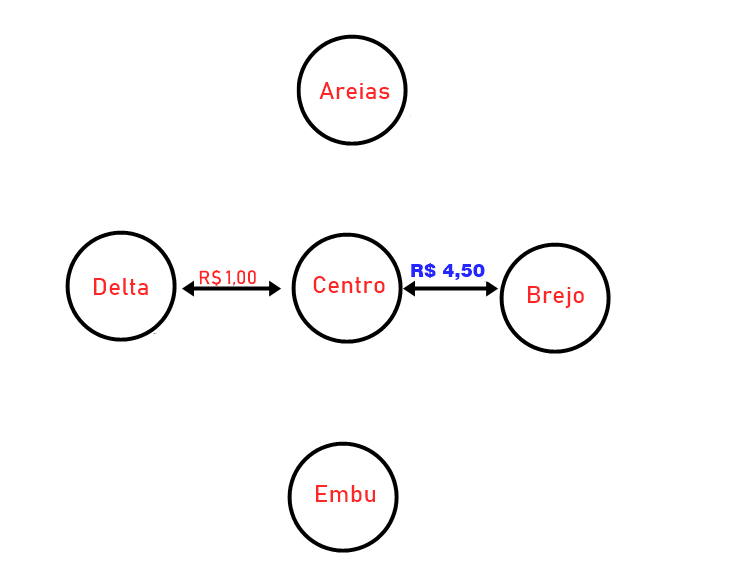
\includegraphics[width=.8\textwidth]{DB3.png}
\label{fig:exampleFig2}
\end{figure}
\begin{equation*}
    \textbf{Total} = R\$1,00 + R\$4,50 = \textbf{R\$5,50}
\end{equation*}

\end{frame}
\begin{frame}{Solução (Viagens de Ônibus)}

%%%%%%%%%%%%%%%%%%%%%%%%%%%%%%%%%%%%%%%%%%%%%%%%%%%%%%%%%%%%%%%%%%%%

\end{frame}

\begin{frame}{Viagens de Ônibus}
\textbf{Questão 10}. Aos domingos o preço da passagem
Centro – Brejo é promocional e custa metade do
preço normal. Nesse caso, qual o menor valor em
passagens para ir de ônibus de Brejo para Delta?

\begin{enumerate}[(A)]
    \item R\$ 2,00
    \item R\$ 4,50
    \item \textbf{R\$ 5,50}
    \item R\$ 6,00
    \item R\$ 9,50
\end{enumerate}
\end{frame}
\begin{frame}{Corrida Robótica}


Uma nova modalidade de corrida de carros foi inaugurada, chamada de Fórmula R, para carros
autônomos (carros sem motorista, dirigidos por robótica). 
\begin{figure}[ht]
\centering
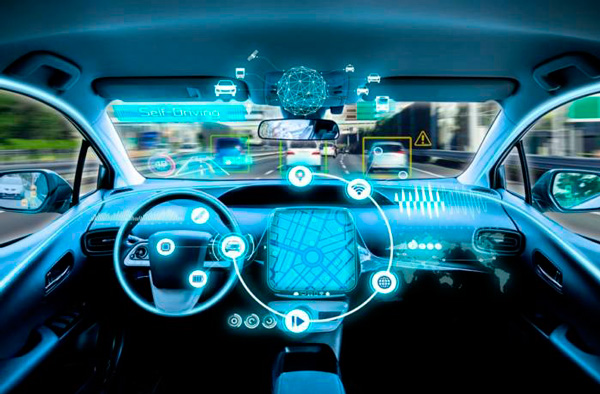
\includegraphics[width=.4\textwidth]{veiculo.jpg}
\label{fig:exampleFig2}
\end{figure}
Na primeira corrida participaram cinco carros, identificados por números, que iniciaram a corrida na seguinte ordem: \textbf{22 (primeiro colocadon os treinos), 16, 27, 31 e 13 (último colocado nos treinos).}
\\ 
\textit{Uma ultrapassagem ocorre quando um carro passa na frente de um outro carro.}
\end{frame}
%%%%%%%%%%%%%%%%%%%%%%%%%%%%%%%%%%%%%%%%%%%%%%%%%%%%%%%%%%%%%%%%%%%%
\begin{frame}{Corrida Robótica}
\textbf{Questão 11}. A seguinte ordem de ultrapassagens ocorreu durante a primeira corrida: o carro 27 ultrapassou o carro 16; o carro 13 ultrapassou o carro 31; o carro 16 ultrapassou o carro 27; o carro 16 ultrapassou o carro 22; o carro 27 ultrapassou o carro 22, e então a corrida terminou. Apenas essas ultrapassagens aconteceram. Qual a ordem de chegada dos carros, do primeiro ao
último colocado?

\begin{enumerate}[(A)]
    \item 27, 16, 22, 13, 31
    \item 22, 27, 16, 31, 13
    \item 22, 16, 27, 31, 13
    \item 16, 22, 27, 13, 31
    \item 16, 27, 22, 13, 31
\end{enumerate}
\end{frame}
%%%%%%%%%%%%%%%%%%%%%%%%%%%%%%%%%%%%%%%%%%%%%%%%%%%%%%%%%%%%%%%%%%%%




\begin{frame}{Corrida Robótica}
Vamos utilizar a cor \textbf{verde} para o carro que irá ultrapassar e \textbf{vermelho} para o que será ultrapassado.
\begin{itemize}


    \item Início da corrida:
        \begin{figure}[ht]
        \centering
        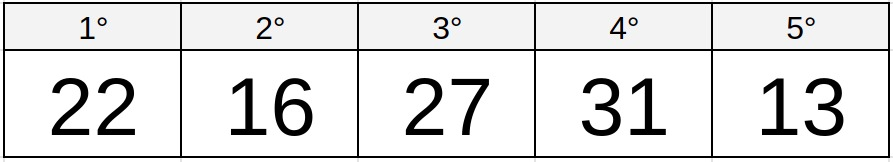
\includegraphics[width=.6\textwidth]{1.jpeg}
        \label{fig:exampleFig2}
        \end{figure}
    \item O carro 27 ultrapassou o carro 16:
        \begin{figure}[ht]
        \centering
        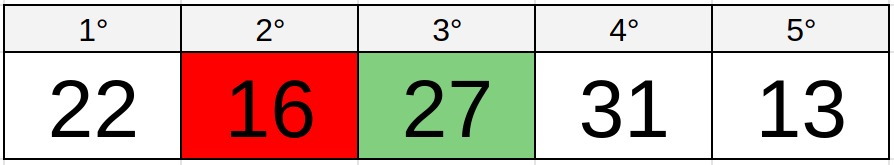
\includegraphics[width=.6\textwidth]{2.jpeg}
        \label{fig:exampleFig2}
        \end{figure}
        \begin{figure}[ht]
        \centering
        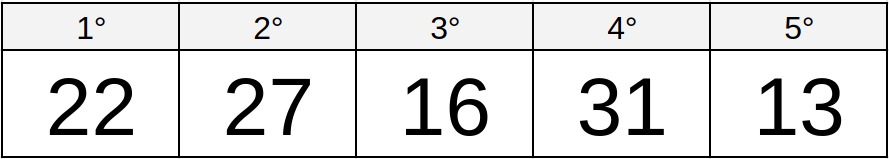
\includegraphics[width=.6\textwidth]{3.jpeg}
        \label{fig:exampleFig2}
        \end{figure}
\end{itemize}
\end{frame}

\begin{frame}{Corrida Robótica}
\begin{itemize}
    \item O carro 13 ultrapassou o casso 31
        \begin{figure}[ht]
        \centering
        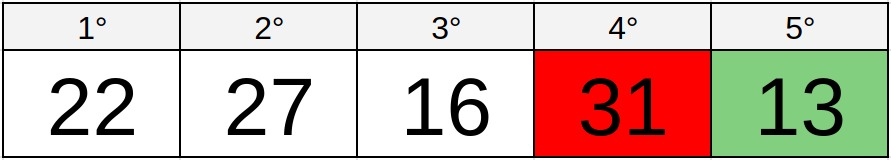
\includegraphics[width=.6\textwidth]{4.jpeg}
        \label{fig:exampleFig2}
        \end{figure}
        \begin{figure}[ht]
        \centering
        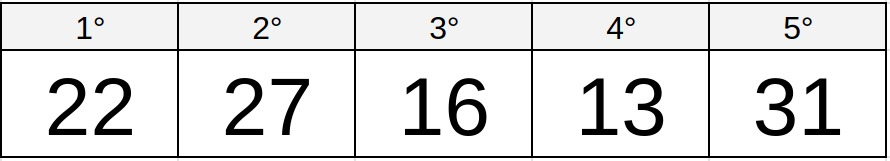
\includegraphics[width=.6\textwidth]{5.jpeg}
        \label{fig:exampleFig2}
        \end{figure}
    \item O carro 16 ultrapassou o carro 27:
        \begin{figure}[ht]
        \centering
        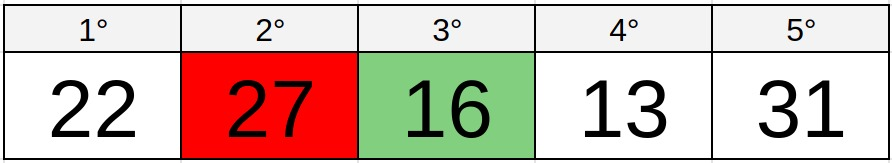
\includegraphics[width=.6\textwidth]{6.jpeg}
        \label{fig:exampleFig2}
        \end{figure}
        \begin{figure}[ht]
        \centering
        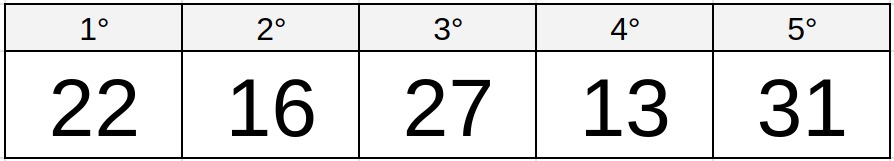
\includegraphics[width=.6\textwidth]{7.jpeg}
        \label{fig:exampleFig2}
        \end{figure}
\end{itemize}
\end{frame}
\begin{frame}{Corrida Robótica}
\begin{itemize}
    \item O carro 16 ultrapassou o casso 22
        \begin{figure}[ht]
        \centering
        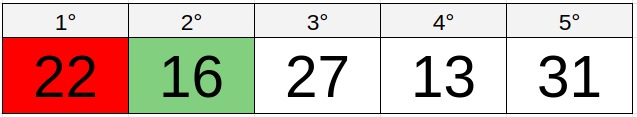
\includegraphics[width=.6\textwidth]{1622.jpeg}
        \label{fig:exampleFig2}
        \end{figure}
        \begin{figure}[ht]
        \centering
        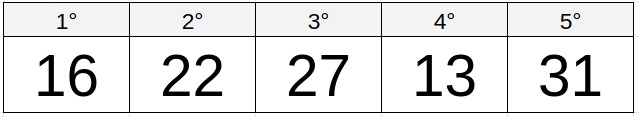
\includegraphics[width=.6\textwidth]{16222.jpeg}
        \label{fig:exampleFig2}
        \end{figure}
    \item O carro 27 ultrapassou o carro 22:
        \begin{figure}[ht]
        \centering
        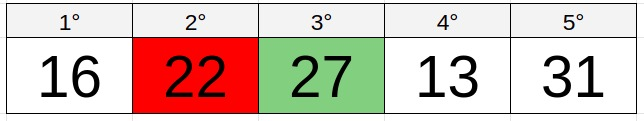
\includegraphics[width=.6\textwidth]{2722.jpeg}
        \label{fig:exampleFig2}
        \end{figure}
        \begin{figure}[ht]
        \centering
        \includegraphics[width=.6\textwidth]{27222.jpeg}
        \label{fig:exampleFig2}
        \end{figure}
\end{itemize}
\end{frame}



%%%%%%%%%%%%%%%%%%%%%%%%%%%%%%%%%%%%%%%%%%%%%%%%%%%%%%%%%%%%%%%%%%%%
\begin{frame}{Solução (Corrida Robótica)}


\textbf{Questão 11}. A seguinte ordem de ultrapassagens ocorreu durante a primeira corrida: o carro 27 ultrapassou o carro 16; o carro 13 ultrapassou o carro 31; o carro 16 ultrapassou o carro 27; o carro 16 ultrapassou o carro 22; o carro 27 ultrapassou o carro 22, e então a corrida terminou. Apenas essas ultrapassagens aconteceram. Qual a ordem de chegada dos carros, do primeiro ao
último colocado?

\begin{enumerate}[(A)]
    \item 27, 16, 22, 13, 31
    \item 22, 27, 16, 31, 13
    \item 22, 16, 27, 31, 13
    \item 16, 22, 27, 13, 31
    \item \textbf{16, 27, 22, 13, 31}
\end{enumerate}
\end{frame}

%%%%%%%%%%%%%%%%%%%%%%%%%%%%%%%%%%%%%%%%%%%%%%%%%%%%%%%%%%%%%%%%%%%%

\begin{frame}{Corrida Robótica}
\textbf{Questão 12}. Na segunda corrida, os carros iniciaram na mesma ordem da primeira corrida (ou seja, 22, 16, 27, 31 e 13). Qual o menor número possível de ultrapassagens durante a segunda corrida, sabendo que os carros terminaram na ordem 13 (vencedor), 22, 16, 31 e 27 (último colocado)?

\begin{enumerate}[(A)]
    \item 5
    \item 6
    \item 7
    \item 8
    \item 9
\end{enumerate}
\end{frame}


%%%%%%%%%%%%%%%%%%%%%%%%%%%%%%%%%%%%%%%%%%%%%%%%%%%%%%%%%%%%%%%%%%%%
\begin{frame}{Solução (Corrida Robótica)}

\begin{itemize}

\pause \item O menor número possível de ultrapassagens durante uma corrida pode ser obtida contando o número de \textbf{inversões} dos carros na largada. 


\pause \item Uma \textbf{inversão} em uma lista de números $a_1, \ldots, a_n$ é um par de números $(a_i,a_j)$ tal que $a_i > a_j$ e $i < j$. 

\pause \item Note que para cada inversão na lista original será necessário uma ultrapassagem.

\end{itemize}

\end{frame}

\begin{frame}{Solução (Corrida Robótica)}

\begin{itemize}

\pause \item Dado a lista de números (22, 16, 27, 31 e 13) temos 5 inversões: \pause (22,16)\pause ,(22,13)\pause,(16,13)\pause,(27,13)\pause e (31,13).

\pause \item Essa contagem pode ser feita de maneira iterativa:

\begin{tabular}{l|p{5cm}}
Lista de carros                 & número de ultrapassagens\\
\hline
(22, 16, 27, 31, 13) & 4 ultrapassagens para o carro 13 ficar primeira posição\\
(13, 22, 16, 27, 31) & 1 ultrapassagens para o carro 16 ficar na segunda posição\\

\end{tabular}
\end{itemize}

\end{frame}


\begin{frame}{Solução (Corrida Robótica)}
\begin{itemize}
    \item Início da corrida
        \begin{figure}[ht]
        \centering
        \includegraphics[width=.6\textwidth]{1.jpeg}
        \label{fig:exampleFig2}
        \end{figure}
        \item Fim da corrida
        \begin{figure}[ht]
        \centering
        \includegraphics[width=.6\textwidth]{fimm.png}
        \label{fig:exampleFig2}
        \end{figure}
        
\end{itemize}
\end{frame}
%%%%%%%%%%%%%%%%%%%%%%%%%%%%%%%%%%%%%%%%%%%%%%%%%%%%%%%%%%%%%%%%%%%%
\begin{frame}{Sessão de Cinema}
Cinco amigas, Ana, Bia, Cris, Duda e Eva querem ir ao cinema, mas a sessão já está quase lotada. Sobraram apenas as cadeiras 1, 2, 3, 4 e 5, todas na primeira fila da plateia.
        \begin{figure}[ht]
        \centering
        \includegraphics[width=.9\textwidth]{cadeiras.png}
        \label{fig:exampleFig2}
        \end{figure}
        Elas compraram os ingressos e agora vão decidir quem senta vizinho a quem. As seguintes restrições devem ser obedecidas:
\begin{itemize}
    \item Ana não quer sentar-se numa cadeira vizinha à cadeira de Bia.
    \item Eva quer sentar-se numa cadeira vizinha à cadeira de Cris.
    \item Cris quer sentar-se ou na cadeira 1 ou na cadeira 5.

\end{itemize}
\end{frame}

%%%%%%%%%%%%%%%%%%%%%%%%%%%%%%%%%%%%%%%%%%%%%%%%%%%%%%%%%%%%%%%%%%%%

\begin{frame}{Sessão de Cinema}
\textbf{Questão 14}. Qual das seguintes alternativas é
sempre verdadeira?
\begin{enumerate}[(A)]
    \item Ana ocupa uma cadeira vizinha à de Duda.
    \item Bia ocupa uma cadeira vizinha à de Eva
    \item Duda ocupa uma cadeira vizinha à de Eva.
    \item Eva ocupa a cadeira 1.
    \item Bia ocupa a cadeira 3.
\end{enumerate}
\end{frame}

%%%%%%%%%%%%%%%%%%%%%%%%%%%%%%%%%%%%%%%%%%%%%%%%%%%%%%%%%%%%%%%%%%%%
\begin{frame}{Solução (Sessão de Cinema)}
\begin{itemize}
    \item \textbf{Supondo} que Cris quer sentar-se na cadeira 1
        \begin{figure}[ht]
        \centering
        \includegraphics[width=.8\textwidth]{nomes1.png}
        \label{fig:exampleFig2}
        \end{figure}
        \pause
        
    \item Eva quer sentar-se numa cadeira vizinha à cadeira de Cris
       \pause
       
       \begin{figure}[ht]
        \centering
        \includegraphics[width=.8\textwidth]{nomes2.png}
        \label{fig:exampleFig2}
        \end{figure}
    \item Ana não quer sentar-se numa cadeira vizinha à cadeira de Bia. \begin{figure}[ht]
        \centering
        \includegraphics[width=.8\textwidth]{nomes 3.png}
        \label{fig:exampleFig2}
        \end{figure}

\end{itemize}
\end{frame}

%%%%%%%%%%%%%%%%%%%%%%%%%%%%%%%%%%%%%%%%%%%%%%%%%%%%%%%%%%%%%%%%%%%%
\begin{frame}{Solução (Sessão de Cinema)}
\begin{itemize}
    \item \textbf{Supondo} que Cris quer sentar-se na cadeira 5
        \begin{figure}[ht]
        \centering
        \includegraphics[width=.8\textwidth]{nomes4.png}
        \label{fig:exampleFig2}
        \end{figure}
        \pause
        
    \item Eva quer sentar-se numa cadeira vizinha à cadeira de Cris
       \pause
       
       \begin{figure}[ht]
        \centering
        \includegraphics[width=.8\textwidth]{nomes5.png}
        \label{fig:exampleFig2}
        \end{figure}
    \item Ana não quer sentar-se numa cadeira vizinha à cadeira de Bia. \begin{figure}[ht]
        \centering
        \includegraphics[width=.8\textwidth]{nome6.png}
        \label{fig:exampleFig2}
        \end{figure}

\end{itemize}
\end{frame}

%%%%%%%%%%%%%%%%%%%%%%%%%%%%%%%%%%%%%%%%%%%%%%%%%%%%%%%%%%%%%%%%%%%%

\begin{frame}{Solução (Sessão de Cinema)}
\textbf{Questão 14}. Qual das seguintes alternativas é
sempre verdadeira?
\begin{enumerate}[(A)]
    \item Ana ocupa uma cadeira vizinha à de Duda.
    \item Bia ocupa uma cadeira vizinha à de Eva
    \item Duda ocupa uma cadeira vizinha à de Eva.
    \item Eva ocupa a cadeira 1.
    \item Bia ocupa a cadeira 3.
\end{enumerate}
        \begin{figure}[ht]
        \centering
        \includegraphics[width=.8\textwidth]{nomes 3.png}
        \label{fig:exampleFig2}
        \end{figure}
         \begin{figure}[ht]
        \centering
        \includegraphics[width=.8\textwidth]{nome6.png}
        \label{fig:exampleFig2}
        \end{figure}

\end{frame}

\begin{frame}{Solução (Sessão de Cinema)}
\textbf{Questão 14}. Qual das seguintes alternativas é
sempre verdadeira?
\begin{enumerate}[(A)]
    \item  \textbf{Ana ocupa uma cadeira vizinha à de Duda.}
    \item Bia ocupa uma cadeira vizinha à de Eva
    \item Duda ocupa uma cadeira vizinha à de Eva.
    \item Eva ocupa a cadeira 1.
    \item Bia ocupa a cadeira 3.
\end{enumerate}
        \begin{figure}[ht]
        \centering
        \includegraphics[width=.8\textwidth]{nomes 3.png}
        \label{fig:exampleFig2}
        \end{figure}
         \begin{figure}[ht]
        \centering
        \includegraphics[width=.8\textwidth]{nome6.png}
        \label{fig:exampleFig2}
        \end{figure}

\end{frame}

%%%%%%%%%%%%%%%%%%%%%%%%%%%%%%%%%%%%%%%%%%%%%%%%%%%%%%%%%%%%%%%%%%%%
\begin{frame}{Sessão de Cinema}
\textbf{Questão 15}. Se Bia ocupa a cadeira 5, qual das seguintes alternativas é sempre falsa?

\begin{enumerate}[(A)]
    \item Eva ocupa a cadeira 2.
    \item Ana ocupa uma cadeira vizinha à cadeira de Eva.
    \item Duda ocupa a cadeira 3.
    \item Ana ocupa a cadeira 3.
    \item Bia ocupa uma cadeira vizinha à cadeira de Duda.

\end{enumerate}
\end{frame}

%%%%%%%%%%%%%%%%%%%%%%%%%%%%%%%%%%%%%%%%%%%%%%%%%%%%%%%%%%%%%%%%%%%%
\begin{frame}{Solução (Sessão de Cinema)}
\begin{enumerate}[(A)]
  \item Ana não quer sentar-se numa cadeira vizinha à cadeira de Bia.
    \item Eva quer sentar-se numa cadeira vizinha à cadeira de Cris.
    \item Cris quer sentar-se ou na cadeira 1 ou na cadeira 5
 \end{enumerate}
 \\
 \\
Se Bia ocupa a cadeira 5, então Cris ocupa a cadeira 1:
 \begin{figure}[ht]
        \centering
        \includegraphics[width=.8\textwidth]{nomes7.png}
        \label{fig:exampleFig2}
        \end{figure}
Segundo a regra \textbf{b}, temos: 
 \begin{figure}[ht]
        \centering
        \includegraphics[width=.8\textwidth]{nomes8.png}
        \label{fig:exampleFig2}
        \end{figure}
\end{frame}
%%%%%%%%%%%%%%%%%%%%%%%%%%%%%%%%%%%%%%%%%%%%%%%%%%%%%%%%%%%%%%%%%%%%
\begin{frame}{Solução (Sessão de Cinema)}
\begin{enumerate}[(A)]
  \item Ana não quer sentar-se numa cadeira vizinha à cadeira de Bia.
    \item Eva quer sentar-se numa cadeira vizinha à cadeira de Cris.
    \item Cris quer sentar-se ou na cadeira 1 ou na cadeira 5
 \end{enumerate}
 \\
 \\

E seguindo a regra \textbf{a}:
        \begin{figure}[ht]
        \centering
        \includegraphics[width=.8\textwidth]{nomes9.png}
        \label{fig:exampleFig2}
        \end{figure}
\end{frame}
%%%%%%%%%%%%%%%%%%%%%%%%%%%%%%%%%%%%%%%%%%%%%%%%%%%%%%%%%%%%%%%%%%%%
\begin{frame}{Solução (Sessão de Cinema)}
\textbf{Questão 15}. Se Bia ocupa a cadeira 5, qual das seguintes alternativas é sempre falsa?

\begin{enumerate}[(A)]
    \item Eva ocupa a cadeira 2.
    \item Ana ocupa uma cadeira vizinha à cadeira de Eva.
    \item Duda ocupa a cadeira 3.
    \item Ana ocupa a cadeira 3.
    \item Bia ocupa uma cadeira vizinha à cadeira de Duda.

        \begin{figure}[ht]
        \centering
        \includegraphics[width=.8\textwidth]{nomes9.png}
        \label{fig:exampleFig2}
        \end{figure}
        
\end{enumerate}
\end{frame}
%%%%%%%%%%%%%%%%%%%%%%%%%%%%%%%%%%%%%%%%%%%%%%%%%%%%%%%%%%%%%%%%%%%%
\begin{frame}{Solução (Sessão de Cinema)}
\textbf{Questão 15}. Se Bia ocupa a cadeira 5, qual das seguintes alternativas é sempre falsa?

\begin{enumerate}[(A)]
    \item Eva ocupa a cadeira 2.
    \item Ana ocupa uma cadeira vizinha à cadeira de Eva.
    \item \textbf{Duda ocupa a cadeira 3.}
    \item Ana ocupa a cadeira 3.
    \item Bia ocupa uma cadeira vizinha à cadeira de Duda.

        \begin{figure}[ht]
        \centering
        \includegraphics[width=.8\textwidth]{nomes9.png}
        \label{fig:exampleFig2}
        \end{figure}
        
\end{enumerate}
\end{frame}

%%%%%%


\end{document}